\documentclass[tikz,border=2pt]{standalone}
\usepackage{amsmath,amssymb}
\usepackage{tikz}

\begin{document}
% A bipartite matching: pairs between two groups (workers and jobs) such that nobody is used
% twice; the thick edges form a maximum matching of size 3.
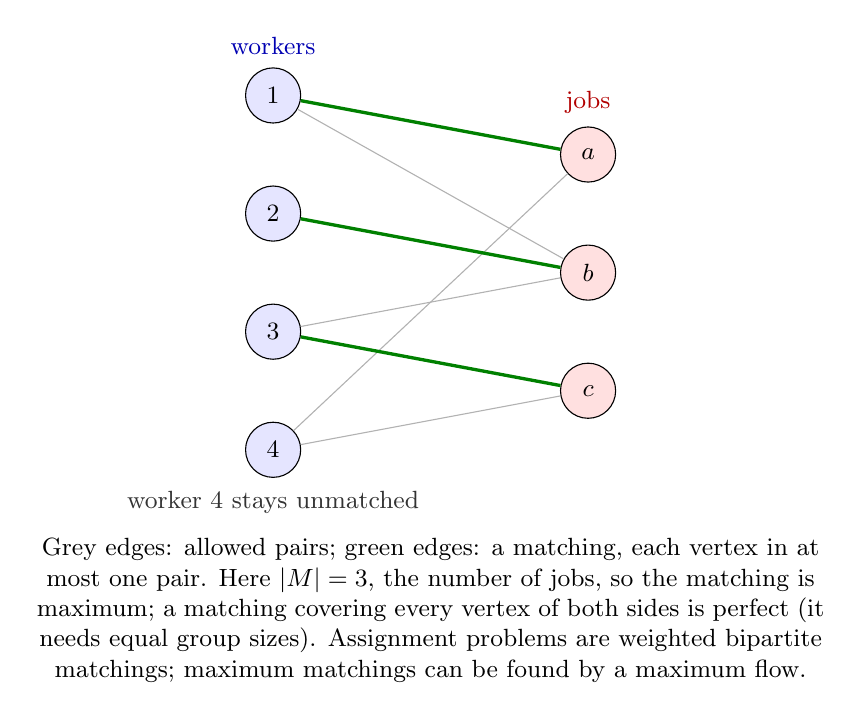
\begin{tikzpicture}[every node/.style={font=\small}, v/.style={draw, circle, fill=blue!10, minimum size=7mm, inner sep=0pt}, w/.style={draw, circle, fill=red!12, minimum size=7mm, inner sep=0pt}]
	\foreach \i in {1,2,3,4} {\node[v] (a\i) at (0,{4.5-1.5*\i}) {$\i$};}
	\foreach \j/\l in {1/a, 2/b, 3/c} {\node[w] (b\j) at (4,{3.75-1.5*\j}) {$\l$};}
	\foreach \i/\j in {1/1, 1/2, 2/2, 3/2, 3/3, 4/3, 4/1} {\draw[gray!60] (a\i) -- (b\j);}
	\draw[green!50!black, very thick] (a1) -- (b1);
	\draw[green!50!black, very thick] (a2) -- (b2);
	\draw[green!50!black, very thick] (a3) -- (b3);
	\node[blue!70!black, anchor=south] at (0,3.4) {workers};
	\node[red!70!black, anchor=south] at (4,2.65) {jobs};
	\node[gray!40!black, anchor=north] at (0,-1.9) {worker $4$ stays unmatched};
	\node[anchor=north, align=flush center, text width=10cm] at (2,-2.5) {Grey edges: allowed pairs; green edges: a matching, each vertex in at most one pair. Here $|M|=3$, the number of jobs, so the matching is maximum; a matching covering every vertex of both sides is perfect (it needs equal group sizes). Assignment problems are weighted bipartite matchings; maximum matchings can be found by a maximum flow.};
\end{tikzpicture}
\end{document}
